% =========================================================================
% Making the Invisible Intelligible
% MSc Thesis — Enrico Vaccari
% Sustainability, Innovation & Technology — Tomorrow University
% =========================================================================

\documentclass[11pt, a4paper, twoside, openright]{book}

% ---------- core packages ----------
\usepackage[utf8]{inputenc}
\usepackage[T1]{fontenc}
\usepackage[english]{babel}
\usepackage{csquotes}
\usepackage{microtype}

% ---------- typography ----------
% Charter is a warm, readable academic serif; switch to lmodern if you prefer
\usepackage{charter}
\linespread{1.15}

% ---------- page geometry (sober, academic) ----------
\usepackage[
    a4paper,
    top=2.8cm,
    bottom=3cm,
    inner=3cm,
    outer=2.5cm,
    headheight=14pt
]{geometry}

% ---------- math & symbols ----------
\usepackage{amsmath, amssymb, amsthm, mathtools}
\usepackage{siunitx}
\sisetup{detect-all}

% ---------- figures, tables ----------
\usepackage{graphicx}
\graphicspath{{figures/}}
\usepackage{booktabs}
\usepackage{caption}
\captionsetup{font=small, labelfont=bf, format=plain}
\usepackage{subcaption}
\usepackage{float}

% ---------- lists, layout ----------
\usepackage{enumitem}
\setlist[itemize]{itemsep=2pt, topsep=4pt}
\usepackage{parskip}

% ---------- headers & footers ----------
\usepackage{fancyhdr}
\pagestyle{fancy}
\fancyhf{}
\fancyhead[LE,RO]{\thepage}
\fancyhead[RE]{\textit{\nouppercase{\leftmark}}}
\fancyhead[LO]{\textit{\nouppercase{\rightmark}}}
\renewcommand{\headrulewidth}{0.4pt}

% ---------- chapter style: sober, no decorative junk ----------
\usepackage{titlesec}
\titleformat{\chapter}[display]
    {\normalfont\Huge\bfseries}
    {\chaptertitlename\ \thechapter}{20pt}{\Huge}
\titlespacing*{\chapter}{0pt}{-30pt}{40pt}

% ---------- hyperlinks ----------
\usepackage[
    colorlinks=true,
    linkcolor=black,
    citecolor=black,
    urlcolor=black,
    bookmarksnumbered=true
]{hyperref}

% ---------- bibliography: APA 7th, via biblatex/biber ----------
\usepackage[
    backend=biber,
    style=apa,
    sortlocale=en_GB,
    natbib=true
]{biblatex}
\addbibresource{references.bib}

% ---------- abbreviations / glossary ----------
% Uncomment if you decide to use a glossary (recommended for AMOC/RAPID/PCA etc.)
% \usepackage[acronym, nonumberlist]{glossaries}
% \makeglossaries
% \input{frontmatter/acronyms}

% ---------- custom commands ----------
\newcommand{\amoc}{AMOC\xspace}  % example, requires \usepackage{xspace}
\usepackage{xspace}

% =========================================================================
\begin{document}

% ---------- front matter ----------
\frontmatter
\pagenumbering{roman}

% ---------- Title page ----------
\begin{titlepage}
    \centering
    \vspace*{2cm}

    {\large\scshape Tomorrow University of Applied Sciences\par}
    {\large MSc in Sustainability, Innovation \& Technology\par}
    {\large Innovation \& Technology Lab\par}

    \vfill

    {\Huge\bfseries Making the Invisible Intelligible\par}
    \vspace{0.6cm}
    {\Large\itshape Machine-learning–derived representations of AMOC instability\\for the public understanding of climate tipping risk\par}

    \vfill

    {\large\itshape Author\par}
    {\large Enrico Vaccari\par}
    \vspace{0.8cm}
    {\large\itshape Supervisor\par}
    {\large Prof.\ Jonathan Costa\par}

    \vfill

    {\large \today\par}
\end{titlepage}
\cleardoublepage

\chapter*{Abstract}
\addcontentsline{toc}{chapter}{Abstract}

% 300–500 words. Write LAST. The order should be:
% (1) the human problem (climate tipping risk is hard to grasp),
% (2) the case study chosen (AMOC) and why,
% (3) the approach (ML as substrate for experiential representation),
% (4) the validation completed so far (flat-manifold, null EWS, anomaly detection),
% (5) the contribution claimed (a transferable method for making invisible
%     systems intelligible, evaluated qualitatively on real participants),
% (6) one sentence on implications.

\textit{[Draft to be written after Discussion is complete.]}

\cleardoublepage

\chapter*{Acknowledgements}
\addcontentsline{toc}{chapter}{Acknowledgements}

\textit{[To be written. Order: supervisor, family/partner, peers, the
RAPID and Copernicus observing communities whose open data made this work
possible.]}

\cleardoublepage


\tableofcontents
\listoffigures
\listoftables

% ---------- main matter ----------
\mainmatter
\pagenumbering{arabic}

\part{Foundations: The Problem and the System}
% =========================================================================
% CHAPTER 1 — INTRODUCTION
% =========================================================================

\chapter{Introduction}
\label{ch:introduction}

\noindent
{\rmfamily\itshape
\begin{tabular}[t]{@{}l@{\hspace{0.3cm}}p{12.5cm}@{}}
\textls[50]{\textbf{Addressed:}} &
\textls[50]{Background \& Context · Personal Mission Alignment · Thesis Statement · Innovation Relevance \& SDG Alignment}
\end{tabular}
}

% -------------------------------------------------------------------------
\section{The Problem: Cognitive Inaccessibility of Complex Climate Systems}
\label{sec:problem-of-knowing}

For three decades, climate communication was guided by a simple assumption: the idea that people fail to act because they lack information, and that better facts would close the gap. However, empirical evidence has consistently challenged this assumption. \citet{kellstedt2008} found that people who knew \emph{more} about climate change often reported \emph{less} concern and a weaker sense of responsibility, even after controlling for politics and demographics. \citet{kahan2015} showed that scientific literacy can widen rather than close disagreement: the most literate people on opposing sides diverge the most when reading the same evidence. Information, it turns out, is filtered through prior beliefs, cultural identity, and the machinery of cognition. The task is not only to state climate science more accurately, but to present it in a form that matches how people actually make sense of it.

There is a much deeper obstacle that sits beneath this one and predates the climate debate. Across two decades of experiments, \citet{sterman2008} found that even highly educated people --- MIT graduate students, engineers, participants trained in mathematics --- reason poorly about systems built on accumulation and flow. \citet{cronin2009} showed it clearly: given the inflow and outflow of a system and asked to sketch the accumulated stock, many participants confused rates with levels and treated a dynamic process as if it were static. These were not people who lacked the mathematics; they had it, and still the static representation defeated them. The implication for climate is direct. Showing CO\textsubscript{2} emissions and atmospheric concentration as two curves does not convey that the second is the accumulation of the first, so audiences systematically underestimate how much inertia the system carries \citep{cronin2009, sterman2008}. Cognitive-load theory explains why: working memory is limited, and a representation that asks the viewer to mentally animate a hidden process imposes a burden that grows with the system's complexity \citep{sweller1988}.
 
These two literatures --- how climate information is interpreted, and how people reason about dynamic systems --- meet at a single conclusion. Communicating a complex climate system is not mainly a problem of accuracy or messaging. It is a problem of \emph{representation}: of finding forms in which the dynamic, multi-scale, potentially non-linear behaviour of such a system becomes something a person can perceive, rather than something they must reconstruct in their head from a static picture.


% -------------------------------------------------------------------------
\section{The Gap and the Proposal}
\label{sec:gap-proposal}
 
This representational problem has been approached from two directions, each strong on its own and rarely joined. Climate-visualisation research has documented, in detail, why conventional formats fail non-specialist audiences --- and has shown that the visualisations people find clearest are often not the ones they understand best \citep{harold2016, kause2021}. Separately, machine learning for climate science has grown rapidly, but almost entirely in a \emph{predictive} role: forecasting, detecting anomalies, improving models for expert users \citep{reichstein2019, sonnewald2021}. What has scarcely been tried is using machine learning not to predict, but to \emph{recover the hidden structure} of a climate system and turn it into a form non-specialists can perceive. The gap this thesis occupies is the intersection of the two: the analytical power of the second, directed at the representational problem named by the first.\footnote{Both literatures are reviewed in full in Chapter~\ref{ch:literature}, which locates the thesis precisely against existing visualisation research, machine-learning applications, and the cognitive-science principles that ground the design.}
 
The thesis proposes an integrative framework built in three stages, each drawing on a different tradition and feeding the next. The first is \emph{analytical}: unsupervised machine learning is applied to observational and reanalysis data, not to forecast, but to recover the latent structure of the system --- a compact set of coordinates that captures its essential dynamics (Chapter~\ref{ch:data_pipeline}). The second is \emph{design-based}: those latent structures are translated into experiential representations, with every design decision grounded in principles from cognitive science, embodied cognition, and information visualisation (Chapter~\ref{ch:translate}). The third is \emph{empirical}: the resulting representations are evaluated against a conventional static baseline through a mixed-methods user study, testing whether they change how non-specialist audiences understand the system (Chapter~\ref{ch:userstudy}). Put simply: machine learning extracts, design translates, evaluation tests.
% -------------------------------------------------------------------------
\section{The Case Study: AMOC as a Test of the Framework}
\label{sec:case-study-amoc}

A framework like this needs a case demanding enough to test it, and the choice is deliberate: the system should carry the very features that make communication hard.\footnote{The AMOC is used only as a test case. This thesis makes no new oceanographic claim and does not contribute to ocean-circulation research; it engages the AMOC solely through the aspects relevant to the representational problem. Its physical foundations --- the governing mechanisms, the Stommel two-box model of bistability, and the formulation of meridional transport --- are quickly touched on in Chapter~\ref{ch:background} for completeness.} The Atlantic Meridional Overturning Circulation (AMOC) is such a system. It is invisible in a strong sense: no surface expression reveals it to the eye, and no everyday experience gives access to it. It spans an ocean basin, so no single location shows its behaviour. It varies over decades to centuries, longer than both human experience and the observational record. It is temporally non-linear and a candidate tipping element, whose substantial weakening could shift the circulation into a different regime with hysteresis \citep{armstrongmckay2022, lenton2008}. This matters because a marked slowdown would reorganise North Atlantic heat transport and reshape the climate of Europe \citep{buckley2016}. Its strength is measured in Sverdrup and observed continuously since 2004 by the RAPID array at \ang{26.5}N \citep{frajkawilliams2021, moat2026}, with the Copernicus GREP reanalysis extending the record further back.
 
The AMOC is the system this thesis studies, but not the one most people picture when they think of climate change. When non-specialists are asked to imagine it, they tend to name visible things --- melting ice, extreme heat, rising seas \citep{oneill2014}. That contrast, between climate systems we can see and those that need instruments and computation to perceive at all, is central to the argument here. The two are not independent. The Greenland Ice Sheet, among the most visible signs of a warming world, is physically coupled to the AMOC: freshwater from Greenland lowers the density of North Atlantic surface water, weakens deep-water formation, and can slow the circulation \citep{boning2016, caesar2018, rahmstorf2015}. What people can see is linked to what they cannot --- and this thesis uses that bridge, from the visible glacier to the hidden current, as the entry point into the invisible system.\footnote{The recent behaviour of the AMOC is itself contested: reconstructions suggest long-term weakening and possible approach to a transition \citep{caesar2018, boers2021, ditlevsen2023}, a reading challenged on methodological grounds \citep{benyami2024}, while the direct RAPID record shows no clear long-term slowdown \citep{moat2026}. This unresolved debate makes clear representation more necessary, not less.}

% -------------------------------------------------------------------------
\section{On the Interdisciplinary Nature of the Work}
\label{sec:positioning}

I began this work driven by a personal mission: \emph{Wisdom Unlocks Awareness, and Awareness Unlocks Agency}. More than a motto, it is the conviction that has guided every decision throughout this journey. I believe that understanding is what gives knowledge the power to move people—not only to know, but to care, and ultimately, to act. People rarely act on a system because they have been told it matters; they act once they grasp it well enough to feel why. This thesis is built at the meeting point of five fields, each carrying part of that problem. Climate science supplies the system, the data, and the standards of evidence. Machine learning supplies the methods that recover hidden structure from data too high-dimensional for the eye --- and stands, here, for a wider belief: that emerging technologies, used responsibly and for people rather than instead of them, can become instruments of understanding, not just engines of prediction. Cognitive science explains why dynamic systems defeat intuition, and what lets a mind find its footing. Information visualisation supplies the principles for turning structure into something perceptible. And science communication sets the final test --- not whether a representation is accurate, but whether it leaves a non-specialist genuinely understanding, in the mind and in the gut, because a decision made with both is one that holds. The contribution lies in none of these fields alone, but in binding them together. Evidence, the computation that reveals it, and the form in which a person finally meets it are usually kept apart; this thesis refuses that separation --- because the future turns on our capacity to understand, together, the systems that will shape it.

% -------------------------------------------------------------------------
\section{Contribution, Innovation Relevance and SDG Alignment}
\label{sec:contribution}

The contribution is mainly methodological. It is not a new finding about the ocean, nor a new machine-learning technique, but a defensible way of connecting the analytical structure of a complex climate system to the perceptual conditions under which non-specialists meet it --- tested against a conventional baseline, so that its value rests on evidence rather than assertion. Positioned against existing work, the approach is distinctive in combining four elements that have not been brought together: recovering a tipping system's latent structure through machine learning, translating it into an experiential representation, grounding each choice in cognitive-science principles, and evaluating the result comparatively.\footnote{Four families of related work --- conventional static visualisation, interactive climate tools, immersive and experiential formats, and data physicalisation --- are examined in Chapter~\ref{ch:literature}. None integrates all four elements above.}
 
The relevance runs on three levels. \emph{Academically}, research on communicating complex climate systems has leaned on preference studies --- which representation feels clearer --- more than on tested comprehension, and experiential formats remain largely unevaluated; this thesis offers a comparative methodology instead of another visualisation. \emph{Institutionally}, it aligns substantively with the United Nations Sustainable Development Goals: primarily \textbf{SDG~13 (Climate Action)}, target~13.3 on education, awareness and capacity \citep{un2015}; secondarily \textbf{SDG~4 (Quality Education)}, in making complex science accessible; and indirectly \textbf{SDG~14 (Life Below Water)}, as the AMOC is part of the ocean system. \emph{Practically}, the framework is built to transfer: the AMOC is one of a family of tipping elements --- ice sheets, the Amazon, permafrost, the monsoon --- that share invisibility, long timescales, non-linearity and high stakes \citep{armstrongmckay2022, lenton2008}. It is a demanding test case for this matter. Before a society can act on a complex system, it must first be able to picture it; this thesis is one contribution to learning how.

% figures/sdg/sdg_alignment.tex
% Three SDG icons this thesis aligns with, shown horizontally.
% Official UN SDG icons — see caption for attribution.
\begin{figure}[!ht]
    \centering
    
\includegraphics[height=4cm]{figures/sdg/sdg4.png}\hfill
    
\includegraphics[height=4cm]{figures/sdg/sdg13.png}\hfill
    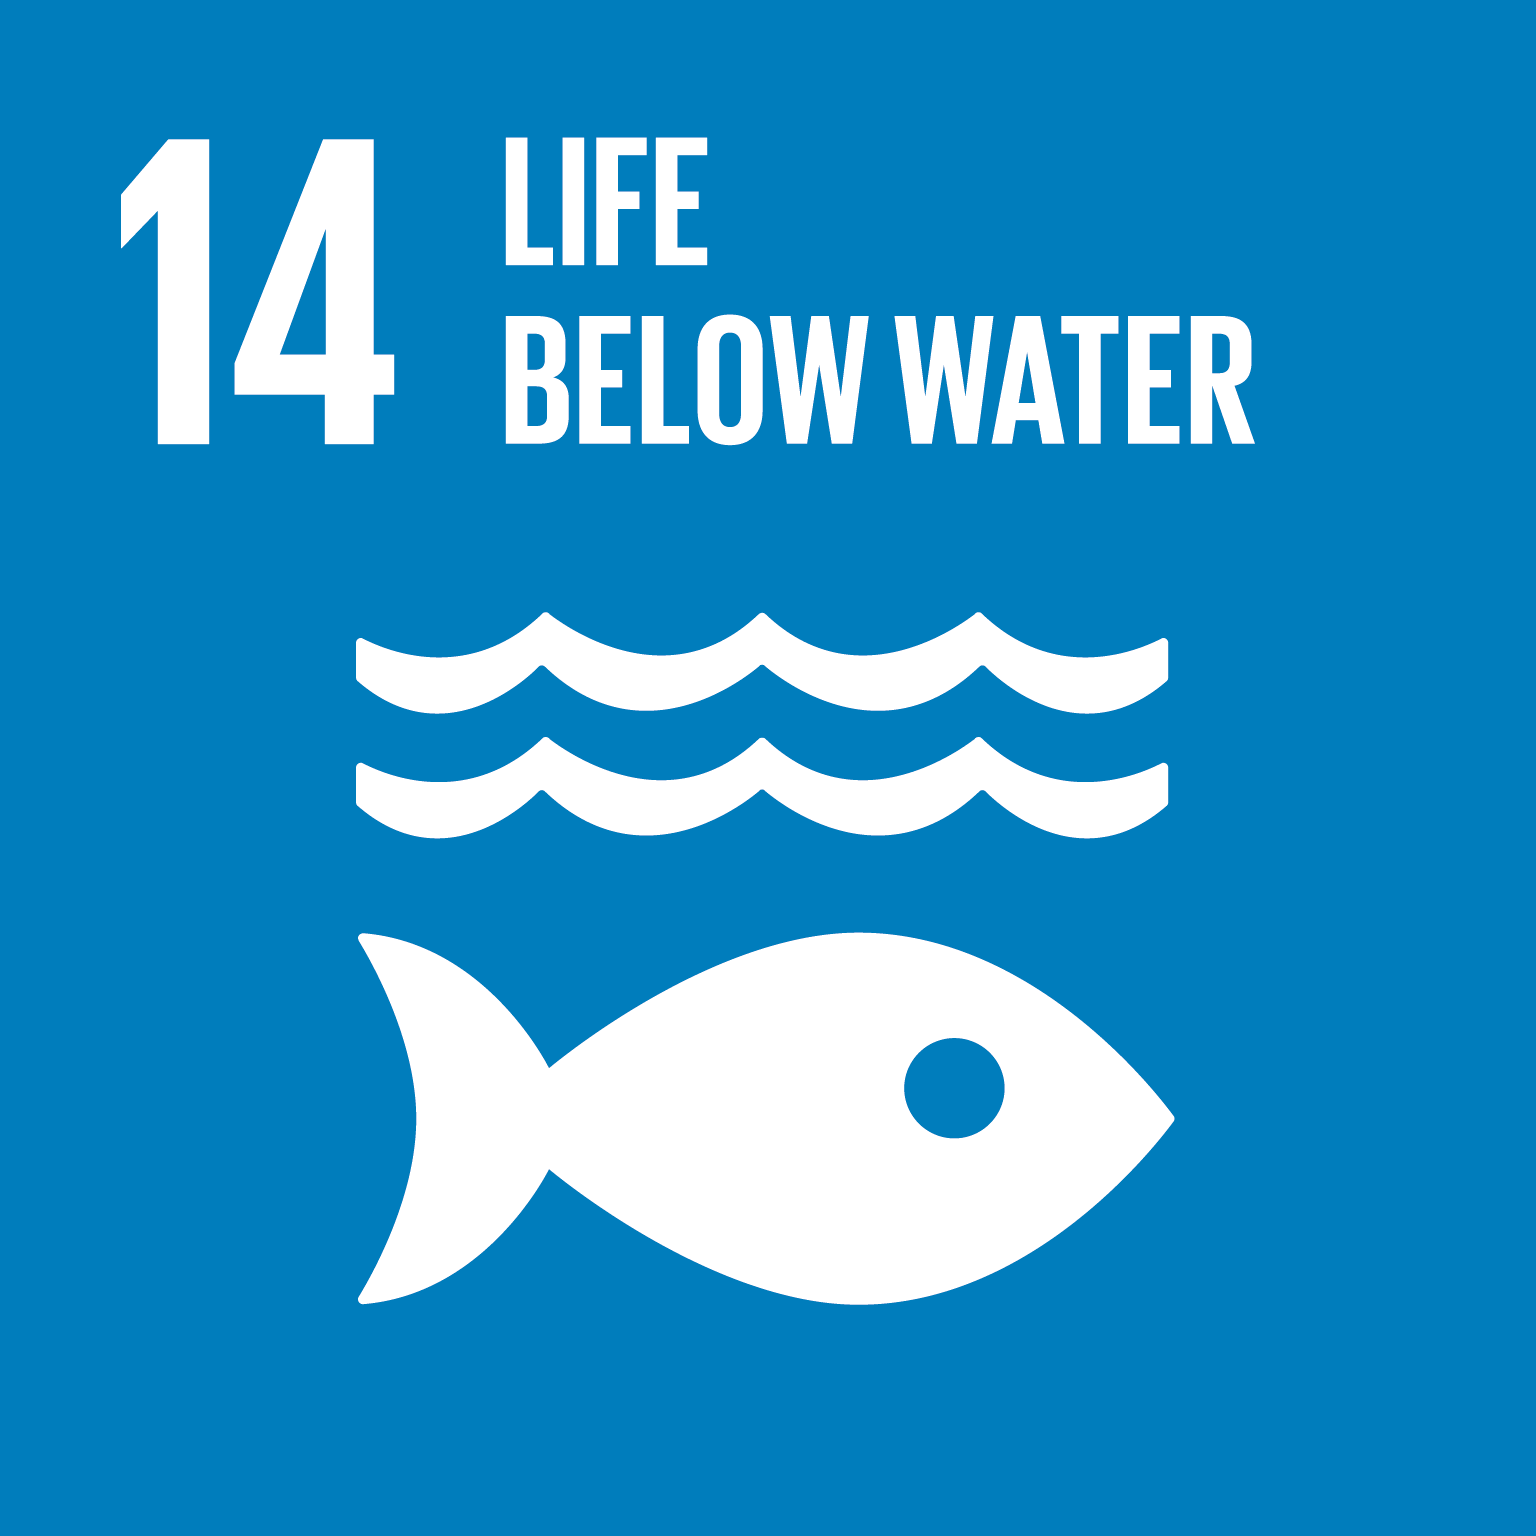
\includegraphics[height=4cm]{figures/sdg/sdg14.png}
    \caption[Sustainable Development Goals addressed by this thesis.]{\textbf{The
    three Sustainable Development Goals this thesis contributes to.} SDG~13
    (Climate Action), in particular target~13.3 on education, awareness and
    capacity; SDG~4 (Quality Education), on making complex knowledge accessible;
    and SDG~14 (Life Below Water), as the AMOC is part of the ocean system.
    Icons \textcopyright~United Nations. The content of this publication has not
    been approved by the United Nations and does not reflect its views.}
    \label{fig:sdg-alignment}
\end{figure}

% -------------------------------------------------------------------------
\section{Roadmap}
\label{sec:roadmap}

The thesis follows the detect--translate--evaluate arc in three parts. 

\textbf{Part~I --- DETECT} sets up the problem and the case: Chapter~\ref{ch:rqs} formalises the research questions, objectives and hypotheses; Chapter~\ref{ch:literature} reviews the relevant literature and locates the thesis within it; Chapter~\ref{ch:background} develops the physical and mathematical apparatus needed to treat the AMOC as an analysable object. 

\textbf{Part~II --- TRANSLATE} documents the constructive work: Chapter~\ref{ch:methodology} specifies the three-stage methodology; Chapter~\ref{ch:data_pipeline} presents the analytical pipeline that recovers the system's latent structure; Chapter~\ref{ch:translate} designs the representational conditions through which that structure is translated. 

\textbf{Part~III --- EVALUATE} closes the loop: Chapter~\ref{ch:userstudy} specifies the user study, Chapter~\ref{ch:results} reports its findings, Chapter~\ref{ch:discussion} interprets them, and Chapter~\ref{ch:conclusion} reflects on limitations, transferability and future work.

\chapter{Research Questions, Objectives and Hypotheses}
\label{ch:rqs}

\textit{[To be ported from the working document, with the corrections we
agreed on: O1.3 reframed as documented future work (LSTM deferred);
O3.2 reframed as a qualitative, exploratory study (N=8--12, think-aloud,
thematic analysis); the umbrella hypotheses H-A and H-B established at
the head, and the technical hypotheses H1--H5 derived from them.]}

% =========================================================================
% CHAPTER 3 — LITERATURE AND MARKET REVIEW
% Section 3.1 — Psychological Barriers to Climate Risk Perception
% =========================================================================

\chapter{Literature and Market Review}
\label{ch:literature}

The literature reviewed in this chapter organises around five strands that together define the intersection at which this thesis positions itself: the psychology of climate risk perception, the cognitive science of dynamic and complex systems, the empirical evaluation of climate visualisation, the strands of data humanism, embodied cognition and immersive analytics, and the applications of machine learning to Earth-system science. Each strand is developed as a compact argument rather than as an inventory of publications; the sixth and final section synthesises them into the specific gap the thesis addresses.

% -------------------------------------------------------------------------
\section{Psychological Barriers to Climate Risk Perception}
\label{sec:psych-barriers}

For much of the late twentieth century, the dominant model of climate communication rested on what became known as the information-deficit hypothesis: the assumption that public inaction on climate change reflected a shortage of accurate scientific information, and that closing the knowledge gap would close the action gap. Two decades of empirical research have not been kind to that assumption. \citet{kellstedt2008} showed, in a representative American survey, that respondents who scored higher on climate knowledge expressed \emph{lower} personal concern about the issue and \emph{lower} sense of responsibility for addressing it, an inverse relationship that persisted after controlling for political affiliation and demographic variables. \citet{kahan2015}, extending this line of work, demonstrated that scientific literacy interacted with cultural worldview to \emph{polarise} rather than converge climate attitudes, so that the most scientifically literate members of opposing cultural groups disagreed with each other more sharply than their less-literate counterparts. The uncomfortable finding of this literature is not that information does not matter but that its effects are mediated by cognitive and cultural machinery which the standard formats of climate communication were not designed to address. What has failed is not the messenger's accuracy but the messenger's understanding of who is listening and how.

The most influential systematic account of this failure remains \citet{stoknes2015}, whose typology of five psychological barriers has been widely adopted in the science-communication literature and has structured much of the applied research that followed. The five barriers, which Stoknes labels the \emph{five~Ds}, are \emph{distance} (climate change is perceived as spatially, temporally and socially remote from everyday experience), \emph{doom} (catastrophist framing triggers avoidance rather than engagement), \emph{dissonance} (the gap between climate belief and daily behaviour is resolved by adjusting the belief rather than the behaviour), \emph{denial} (self-protective disengagement from information experienced as threatening) and \emph{identity} (climate positions function as markers of group belonging, making the acceptance of new information contingent on its compatibility with prior identification). The five barriers do not operate independently; \citet{vanderlinden2015} document their interlocking action empirically and argue that effective communication requires addressing them jointly rather than sequentially. The finer-grained segmentation offered by \citet{leiserowitz2021}, in the long-running \emph{Six~Americas} study of the Yale Program on Climate Change Communication, shows that publics stratify into psychologically coherent audiences whose barriers activate differently, so that no single communicative strategy can serve all of them at once. The tempting inference --- that better graphs might solve this --- is not supported by the evidence the following section examines.

The reason conventional visualisation has failed to dissolve the barriers identified by Stoknes and his successors is structural, not aesthetic. \citet{cornerclimate2015}, drawing on empirical work conducted by the Climate Outreach organisation in the United Kingdom, showed that the imagery most frequently used to communicate climate change --- polar bears, smokestacks, calving glaciers, temperature curves --- either reinforces the very psychological distance the communicators hope to close or activates the doom response that suppresses engagement. \citet{nicholsoncole2005}, in what remains a foundational study of the perceptual reception of climate visuals, demonstrated that participants presented with standard scientific climate imagery reported a paradoxical combination of concern and detachment: the imagery made the phenomenon feel real, but it also made it feel finished, already someone else's problem, cognitively closed. The recent review of \citet{ojala2023} synthesises a decade of subsequent work on affective responses to climate communication and concludes that formats which do not offer the reader an active role in relation to the information consistently underperform formats that do. Adding more precision to a line graph does not open such a role; the graph's implicit rhetoric of \emph{here is the fact} leaves the reader with nowhere to stand.

The direction in which the more recent literature has begun to point is towards representational forms that treat the reader as an active participant in the construction of meaning rather than as the passive recipient of an authoritative image \citep{marlon2019, ojala2023}. This shift has taken several forms: narrative-based communication that embeds climate information in stories with which readers can identify \citep{morris2019}, visualisation practices that explicitly invite exploration and interpretation rather than mere reading \citep{cornerclimate2015} and, at the more experimental end, representational practices grounded in embodied and interactive cognition to which this thesis contributes, and which the fourth section of this chapter (§\ref{sec:embodied-viz}) develops in detail. The psychological literature identifies the problem to which the representational literature has yet to find an adequate answer, and the case made in this thesis is that machine learning, treated not as a predictive instrument but as a substrate for representation, offers one path through which that answer might be pursued.

% -------------------------------------------------------------------------
\section{The Cognitive Science of Dynamic and Complex Systems}
\label{sec:cognitive-science}

The psychological literature reviewed in the previous section identified the cultural and affective barriers through which climate information is filtered before it reaches interpretation. The cognitive-science literature reviewed here identifies a barrier of a different kind, prior to filtering and independent of it: the structural limits of the human mind in reasoning about systems whose behaviour is governed by accumulation, feedback and delay. The claim developed in this section is that these limits are not defects of education which better teaching could remedy but stable features of human cognitive architecture, and that any representational strategy which ignores them will fail regardless of how psychologically well-tuned it might be.

The most systematic body of evidence for this claim comes from the work of \citet{sterman2008}, whose two decades of experimental studies have consistently shown that even mathematically literate adults --- graduate students at MIT, engineering professionals, participants with formal training in calculus and dynamics --- make systematic errors when asked to reason about elementary stock-and-flow systems. The experimental design is deceptively simple. Participants were shown a scenario in which atmospheric CO\textsubscript{2} rises gradually and stabilizes at 400~ppmv by 2100 (Figure~\ref{fig:sterman-scenario}), together with the historical trajectory of anthropogenic emissions and the current rate of net removal by oceans and biomass (Figure~\ref{fig:sterman-task}). They were then asked to sketch the emissions path consistent with stabilization. As Figure~\ref{fig:sterman-response} illustrates, 84\% of respondents produced trajectories that violate mass balance: rather than reasoning about the relationship between inflow and outflow, they matched the shape of the output to the shape of the input, keeping emissions well above removal while expecting the stock to stabilize.

% ============================================================
% Sterman (2008) climate stabilization task -- original figures
% extracted from the Science article as vector PDF crops.
%
% Requires the three PDF files in the figures/ folder:
%   sterman_scenario.pdf, sterman_task.pdf, sterman_response.pdf
% (\graphicspath{{figures/}} is already set in main.tex)
% ============================================================

\begin{figure}[htbp]
    \centering
    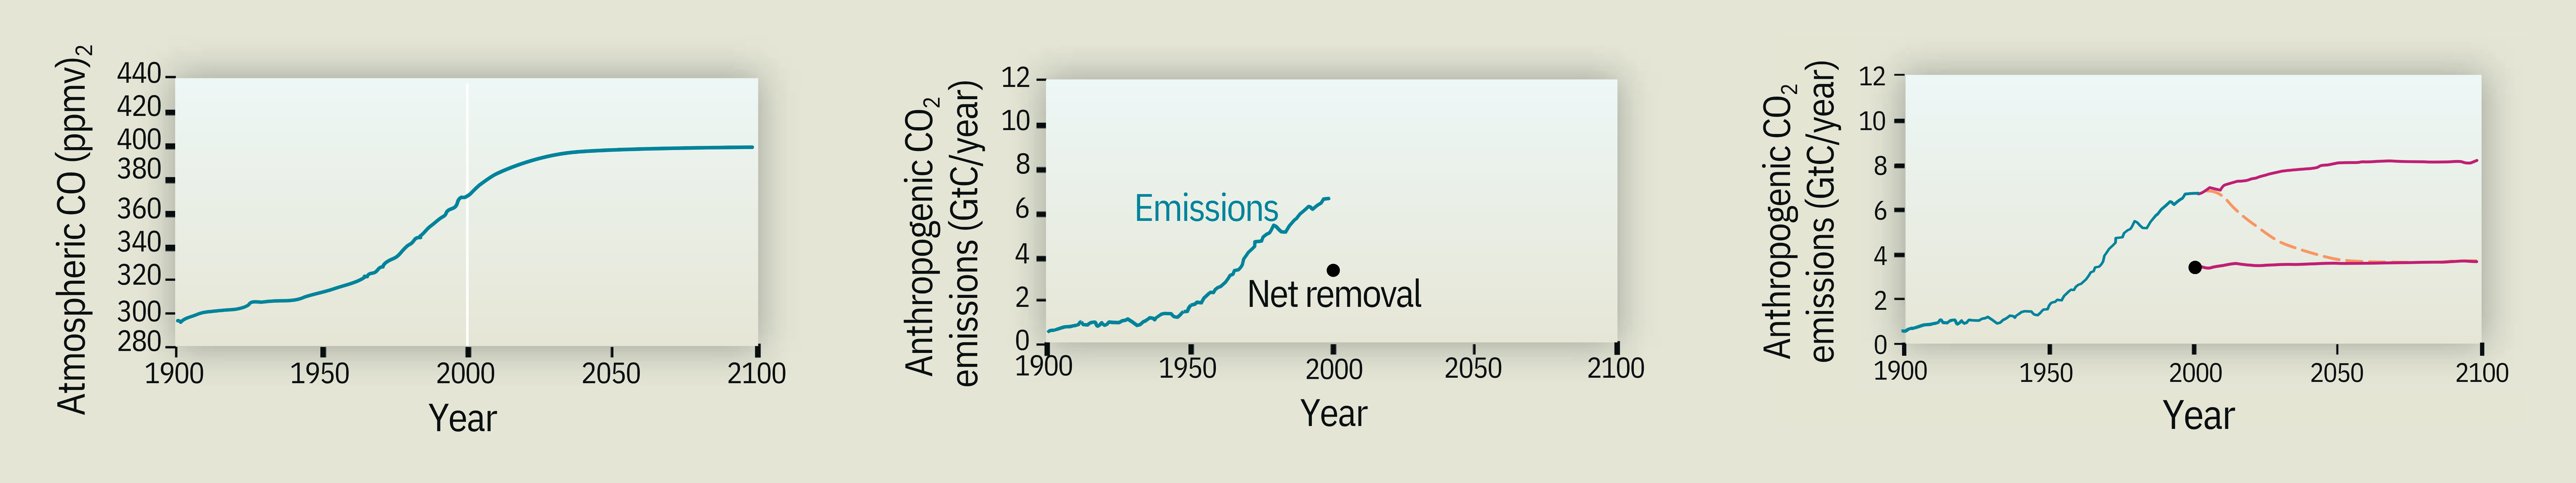
\includegraphics[width=\textwidth]{sterman_panel.png}
    \caption[The climate stabilization task]{The climate stabilization
    task. (a)~The scenario presented to participants: atmospheric
    CO\textsubscript{2} concentration rises gradually to 400~ppmv and
    stabilizes by 2100. (b)~The stock--flow information provided:
    anthropogenic CO\textsubscript{2} emissions from 1900 to 2000 (the
    inflow) and current net removal by oceans and biomass (the
    outflow), with emissions roughly double net removal. (c)~A typical
    response: participants erroneously sketch future emissions that
    match the shape of the CO\textsubscript{2} trajectory
    (pattern-matching heuristic), while mass balance requires emissions
    to fall until they equal net removal (dashed line). Reprinted from
    \citet{sterman2008}.}
    \label{fig:sterman-panel}
\end{figure}

\citet{cronin2009} demonstrated the finding in its starkest form: participants shown a graph of the inflow and outflow of some quantity into a stock were asked to sketch the trajectory of the stock itself, a task equivalent to visually integrating the difference between two curves. Even in scenarios simplified to the point of triviality, the majority produced trajectories that confused rates with levels, mistook peaks in the flow for peaks in the stock and treated the dynamic system as if it were static. The pattern was not distributed randomly across the participant pool; it appeared in the responses of participants who had scored highly on prior tests of mathematical competence and who had, in principle, the technical apparatus to solve the problem correctly. What the study documented was not a failure of arithmetic but a failure of representation --- the mind, given only a graph, does not spontaneously construct the dynamic scenario the graph is meant to depict. The implication for climate communication is direct and uncomfortable: presenting CO\textsubscript{2} emissions and CO\textsubscript{2} concentrations as parallel curves does not communicate that the second is the integral of the first, and readers of the graph will systematically underestimate the inertia of the system \citep{sterman2008}.

A second, converging line of evidence comes from cognitive-load theory as developed by \citet{sweller1988} and extended over three decades of subsequent research \citep{swellervanmerrienboer2019}. The theory rests on a well-documented empirical fact: working memory, the mental resource in which active reasoning occurs, has a strictly limited capacity, and any representational format which requires the reader to hold multiple relationships in working memory simultaneously will produce comprehension errors that scale with the number of relationships. Static visualisations of dynamic systems --- an ensemble spaghetti plot, a set of stacked time series, an isocontour map of projected change --- ask the reader to mentally animate what the visualisation cannot animate directly, to hold in mind the transitions between frames the visualisation cannot show, to construct an internal simulation of a process the graph depicts only in its final state. The cognitive load imposed by this reconstruction is high, and it is imposed \emph{in addition} to the load of understanding the domain itself. The failures of comprehension that result are not deficiencies of the reader; they are predictable consequences of asking working memory to do work for which it does not have capacity. \citet{ware2021}, integrating cognitive-load theory with perceptual research on visual attention, argues that the design of any communicative visualisation must minimise this internal-simulation demand by making the dynamic structure of the system perceptually available in the representation itself.

The third strand of evidence gestures towards the direction in which the following sections will develop. \citet{tversky2019}, in a synthesis of four decades of research on spatial and mental representations, argues that human cognition of complex processes is fundamentally spatial in character: the abstract relationships that constitute a dynamic system are understood through analogy to bodily, spatial and kinaesthetic schemas that the mind already inhabits. This finding is more than a fact about mental imagery; it identifies the cognitive substrate through which any representation of a complex system must be received in order to be understood at all. If systems like the AMOC are structurally dynamic, and human reasoning about dynamic systems is spatially embodied, then the representational strategies most likely to succeed are those which enrol the reader's spatial and kinaesthetic cognition in the reconstruction of the dynamic. This proposition, which the next section develops through the literature on embodied cognition and data physicalisation, is not offered here as a conclusion but as the hypothesis under which the remainder of this chapter is organised.

% -------------------------------------------------------------------------
\section{Empirical Evaluation of Climate Visualisation}
\label{sec:empirical-viz}

The two previous sections established, on the one hand, the psychological and cultural barriers that filter climate information before it reaches interpretation and, on the other hand, the structural limits of cognition that shape what any representation can hope to communicate. This section turns from theory to evidence and asks what has actually been measured about the reception of climate visualisations, and where the resulting empirical literature is thin. The picture that emerges is one of a field methodologically asymmetric: rich in studies of what audiences \emph{prefer} among alternative visualisations and sparse in studies of what audiences actually \emph{understand} when they view them. This asymmetry, more than any single deficit of aesthetics or interactivity, defines the gap this thesis positions itself to address.

The most systematic mapping of the state of the field is offered by \citet{harold2016}, whose review examined the literature on climate-data visualisation against what is known from cognitive and perceptual science about non-expert visual processing. Their central finding is that the standard formats used to communicate climate change --- line graphs of global mean temperature, choropleth maps of projected change, ensemble spaghetti plots, tornado diagrams of sensitivity --- are mismatched to the cognitive resources of the audiences they are meant to inform, and that the mismatch is documented not only in laboratory studies with student participants but in the interpretive errors made by policy audiences with substantial technical training. The finding is corroborated by \citet{mcmahon2015}, whose study of how policy actors interpret IPCC visualisations demonstrated that even trained readers systematically underestimate uncertainty ranges depicted through shaded envelopes and misread ensemble spread as evidence of disagreement rather than as a structural feature of the projection. The specifically visual literature converges with the psychological literature reviewed in §\ref{sec:psych-barriers}: what has failed is not the accuracy of the visualisations but their compatibility with the perceptual machinery through which they are received. \citet{retchless2016}, in a controlled study of alternative encodings for climate uncertainty on choropleth maps, showed that the encodings most commonly used in scientific practice --- bivariate colour schemes and stippled overlays --- produced the poorest comprehension among non-specialist participants, while encodings borrowed from cartographic design traditions performed measurably better. The finding is significant not because it identifies a superior encoding but because it establishes that alternatives exist and that they can be evaluated empirically, a claim which much of the visualisation-design literature makes only in principle.

The more troubling structural finding of the field, however, is what \citet{kause2020} identifies as the persistent gap between preference and comprehension. Their study, one of the few that measured both variables in the same participants, demonstrated that the visualisations participants \emph{preferred} --- those they rated as clearest, most engaging and most trustworthy --- were not the same visualisations that produced the highest measured comprehension of the underlying phenomenon. Participants preferred formats that felt familiar and confident; they understood formats that were structurally aligned with the dynamic being depicted, whether or not they preferred them. A subsequent extension of the work \citep{kause2021} documented the same divergence for the specific case of climate uncertainty, showing that intuitive-seeming icon arrays and confidence bars produced overconfident interpretation while less intuitive but structurally faithful frequency representations produced calibrated interpretation. The methodological consequence is direct and rarely stated: the dominant tradition of preference-based evaluation in the visualisation literature is measuring the wrong variable. Preference is not comprehension, and optimising representations for preference alone risks constructing what \citet{sheppard2015} has called \emph{consoling visualisations} --- images that are received warmly and understood poorly.

The gap in the empirical literature that this thesis addresses can now be stated with precision. Comprehension studies of climate visualisation exist but are outnumbered by preference studies by roughly an order of magnitude, and among the comprehension studies that exist almost none has evaluated experiential or embodied representational formats against conventional graphic ones \citep{harold2016, sheppard2015}. Where comparative studies of alternative formats have been conducted, they have almost always relied on quantitative comprehension tests with population-level inference as their epistemic goal, an approach appropriate for well-defined comprehension outcomes but poorly suited to the exploratory investigation of how non-specialists articulate their understanding of a system for the first time. The methodological space this thesis occupies --- a qualitative, exploratory comparison of three representational conditions using think-aloud protocols and thematic analysis --- is not a replacement for those quantitative traditions but a complement to them, appropriate to a stage of research in which the phenomenon of interest is the \emph{articulation of understanding} itself, and where the depth of interpretive engagement matters more than the breadth of statistical inference \citep{braunclarke2006, smithmcgannon2018}. The evidence base into which this thesis reports is the one identified by the empirical literature as most thinly populated, and it is populated using the methodology the empirical literature identifies as best fit for the question being asked.


% -------------------------------------------------------------------------
\section{Data Humanism, Embodied Cognition and Immersive Analytics}
\label{sec:embodied-viz}

The three previous sections defined the problem this thesis addresses through the successive lenses of psychology, cognitive science and empirical visualisation research. This section turns to the traditions in which the problem's response has begun to take shape. Three related lines of work --- the philosophical account of embodied cognition, the practice of data humanism and physicalisation and the emerging field of immersive analytics --- have converged over the past two decades on a proposition that runs against the mainstream of scientific visualisation: that the intelligibility of complex information depends on the reader's active bodily and perceptual engagement with it, and that representational forms which do not enrol the body and the senses systematically underperform forms that do. Each of the three traditions arrives at this proposition from a different direction, and their convergence provides the theoretical scaffolding on which the design work of Chapter~\ref{ch:translate} is built.

The philosophical grounding of the position was articulated most systematically by \citet{lakoff1999}, whose work on embodied cognition argues that the abstract concepts through which humans reason about complex systems are not disembodied logical structures but extensions of the bodily and spatial experience that human cognition originally evolved to handle. Concepts such as \emph{acceleration}, \emph{feedback}, \emph{stability} and \emph{tipping} are understood, on this view, through the extension of kinaesthetic schemas that the mind has already inhabited --- the sense of a body speeding up, the sense of a movement returning to itself, the sense of a footing that holds, the sense of a footing that gives way. \citet{kirsh2013} provided empirical support for this position in a series of experimental studies showing that participants who were allowed to gesture and move while reasoning about complex processes performed measurably better than participants restricted to inspection of static representations. The finding held across problem types --- mathematical, mechanical and dynamical --- and its consistency has since supported a growing body of design research arguing that representations of complex systems should be understood not as pictures to be viewed but as environments to be inhabited \citep{tversky2019, hurtienne2011}. The implication for climate visualisation is not that graphs should be replaced by simulations but that any visualisation of a system whose reader is expected to reason about dynamic behaviour must offer the reader a form of embodied engagement with the dynamic, whether kinaesthetic, exploratory or perceptual, that inert graphic formats do not provide.

The design tradition that has developed most concretely from this proposition is the practice of \emph{data physicalisation}, defined by \citet{jansen2015} as the construction of physical artefacts whose geometry and material properties encode information for exploration through touch, sight and sometimes sound. The tradition emerged partly in reaction to the perceived limitations of purely visual representation and partly from the design-research community's engagement with tangible interaction \citep{ishii1997}, and it has since produced both craft objects intended for public engagement and rigorous experimental studies comparing physicalisations against equivalent screen-based visualisations. \citet{moere2010} showed, in one of the earliest such comparisons, that participants working with data physicalisations recalled the represented information with greater accuracy and retained it longer than participants working with equivalent bar charts, a finding that has since been extended across data types and modalities \citep{jansen2015}. Parallel to this technical tradition, the practice of \emph{data humanism} associated with the work of Giorgia Lupi \citep{lupi2017} and colleagues at Accurat, Pentagram and Domestic Data Streamers has argued that scientific data communication has been dominated by an aesthetic of dispassionate abstraction that treats the reader as a rational information processor rather than as an embodied and emotional being. The data-humanist alternative --- often executed as hand-drawn or richly illustrated visualisations that foreground authorial voice, imperfection and narrative --- has been received with mixed reactions in the scientific-visualisation literature, but the empirical case for its central claim is stronger than its stylistic surface suggests. Studies of narrative visualisation \citep{segel2010} and of visual explanations grounded in personal experience \citep{morris2019} document consistently that representations which acknowledge the reader as a participant produce measurably deeper engagement than representations that maintain the fiction of a view from nowhere.

The third convergent tradition, more recent and more technically ambitious, is the field of \emph{immersive analytics} as consolidated in the survey volume by \citet{marriott2018}. The field takes as its premise that the immersive display technologies now becoming accessible --- head-mounted virtual reality, augmented reality, large-format wall displays and spatially-aware three-dimensional interfaces --- offer representational affordances that the two-dimensional screen cannot match, and that these affordances are particularly well-suited to data whose structure is inherently spatial, dynamic or multidimensional. Immersive analytics is distinct from earlier scientific visualisation in its explicit orientation towards \emph{analysis by exploration}: rather than presenting a finished view of a dataset, the immersive representation invites the analyst to move through the data, to change viewpoint, to select and to compare, in ways that leverage the same embodied cognitive resources identified by Lakoff and Kirsh \citep{chandler2015}. Empirical evaluations of immersive analytics for scientific data are still limited in number, and the strongest current evidence concerns tasks involving three-dimensional spatial structure and temporal dynamics rather than more abstract representations of complex systems. But the theoretical alignment between immersive analytics and the cognitive-science literature reviewed in §\ref{sec:cognitive-science} is direct, and the practical accessibility of the underlying technologies --- browser-based WebGL for interactive rendering, the Web Audio API for real-time sonification --- has now brought immersive-analytic design within reach of individual research projects at the scale of a Master's thesis. This thesis takes a modest but deliberate step into that space, treating the browser as a medium for embodied representation rather than as a delivery channel for visualisations that could as easily have been printed.

Taken together, the three traditions reviewed in this section support a claim that will structure the remainder of the thesis: the difficulty of communicating complex climate systems to non-specialist audiences is not addressable by refinement within the conventional-visualisation paradigm, and the direction in which the empirical, cognitive and design-research literatures collectively point is one that treats the reader as an active, embodied participant in the construction of understanding. The design of the three representational conditions in Chapter~\ref{ch:translate} is grounded in this claim, and the design decisions made there are defended through the perceptual and cognitive commitments this section has articulated.

% -------------------------------------------------------------------------
\section{Machine Learning for Climate and Earth-System Science}
\label{sec:ml-climate}

The four preceding sections established the representational problem this thesis addresses and the theoretical traditions in which its response is grounded. This section turns to the fifth strand of the literature: the applications of machine learning to climate and Earth-system science, which supply the analytical substrate on which the representational work of Chapter~\ref{ch:translate} is built. The characterisation offered here is not comprehensive; the field is now vast and has been surveyed elsewhere \citep{reichstein2019, sonnewald2021, irrgang2021}. The purpose of this section is more specific: to identify the dominant agenda that has shaped the machine-learning-for-climate literature over the past decade and to locate, against that agenda, the alternative role for machine learning that this thesis undertakes.

The dominant agenda has been broadly \emph{predictive} in orientation. The most cited applications of machine learning to Earth-system data fall into four families: probabilistic short-range forecasting of climate variables through recurrent and convolutional architectures \citep{sonnewald2021, weyn2020}, anomaly detection and event characterisation in observational streams \citep{ham2019}, subgrid-scale parameterisation of physical processes in numerical models \citep{rasp2018, brenowitz2020} and statistical downscaling of coarse-resolution model output to regional scales \citep{vandal2019}. The AMOC-specific literature reflects the same distribution: a growing body of work applies machine-learning techniques to detect early-warning signals in observational and reconstructed transport records \citep{boers2021, ditlevsen2023, benyami2024}, to forecast short-range variability from surface indicators \citep{lu2024} and to identify latent dynamical modes in ensemble reanalyses \citep{sonnewald2019}. The field has developed rapidly, has produced results of substantive scientific value and has established a set of methodological conventions --- benchmark datasets, evaluation protocols and reporting standards --- that are now recognisable across the community. The point relevant here is not that this agenda is misconceived; the point is that it is oriented, almost without exception, toward the production of \emph{new scientific findings for expert audiences}, and that the very success of this orientation has left an adjacent question comparatively unexplored.

The adjacent question concerns what machine learning contributes when the goal is not to produce a new scientific result but to make an existing scientific object \emph{intelligible to non-specialists}. The distinction is worth stating precisely because it is easy to lose. A recurrent neural network trained to forecast the AMOC transport strength six months in advance produces a new quantitative capability, evaluated against a ground-truth held-out record and reported in units --- correlation coefficient, root-mean-square error, calibration score --- that the climate-science community shares. A dimensionality-reduction analysis of the same record produces a latent representation whose value cannot be evaluated in those terms because it does not answer the same kind of question. It answers, instead, a question about \emph{structure}: what are the small number of coordinates that account for most of the record's variability, and what do those coordinates mean physically? The analytical work reported in Chapter~\ref{ch:detect} is of the second kind, and the design work of Chapter~\ref{ch:translate} rests on it. The claim that emerges is not that the AMOC vertical manifold has a novel low-dimensional structure --- the finding is consistent with what oceanographers have understood about the meridional overturning for decades \citep{hannachi2007, buckley2016} --- but that this structure, once recovered and characterised, can serve as the coordinate system through which the AMOC is made available to non-specialist perception. The role of machine learning here is not predictive but \emph{representational}: it produces a substrate on which representational work can be conducted, rather than a forecast whose accuracy is the object of evaluation.

The literature that has treated machine learning in this second, representational role is comparatively thin, but it is not empty. \citet{iten2020}, working in fundamental physics rather than climate science, argued that the latent representations recovered by unsupervised networks can be treated as legitimate epistemological objects --- as ways in which a computational system \emph{proposes} a physical variable that a human interpreter can then examine and name. \citet{camps2019} extended a related argument to seismology, using autoencoder representations of earthquake waveforms as the basis for interactive exploration by non-specialist audiences. In the visualisation-research community, \citet{sacha2018} developed a framework for what they called \emph{visual analytics with machine learning}, in which the model's latent representation is not the final product but the substrate through which the human analyst constructs understanding. The extension of this framework from expert analytics to public communication --- from analyst interfaces to representational artefacts for non-specialists --- has been proposed occasionally in the visualisation literature \citep{munzner2014, cabrera2023} but has been implemented in the climate-communication literature almost nowhere. The specific proposition that this thesis pursues --- that the latent representations recovered from an invisible climate system can be translated into experiential representations legible to non-specialist audiences --- is coherent with the theoretical traditions reviewed in §\ref{sec:embodied-viz} and with the emerging visual-analytics tradition surveyed here, but its systematic empirical development in the climate-communication context has not yet been attempted. The gap this thesis addresses is defined at that intersection.

% -------------------------------------------------------------------------
\section{Synthesis: The Intersection This Thesis Occupies}
\label{sec:literature-synthesis}

Read as a single argument, the five strands of literature reviewed in this chapter converge on a proposition that no single strand articulates on its own. The psychological literature reviewed in §\ref{sec:psych-barriers} establishes that the reception of climate information is filtered through documented cognitive and cultural barriers which conventional formats not only fail to address but occasionally reinforce. The cognitive-science literature reviewed in §\ref{sec:cognitive-science} demonstrates that these barriers are compounded by structural limits on the human capacity to reason about accumulation, feedback and delay from static visual representations. The empirical visualisation research reviewed in §\ref{sec:empirical-viz} documents that the standard formats of climate communication have been evaluated primarily through preference studies rather than through comprehension studies, and that comprehension gains from alternative formats remain largely uncharted. The literatures on embodied cognition, data physicalisation and immersive analytics reviewed in §\ref{sec:embodied-viz} identify the theoretical and design traditions in which the response to this cluster of limitations has begun to take shape, but their application to climate communication has been sporadic and their systematic evaluation on specific climate systems almost absent. The machine-learning-for-climate literature reviewed in §\ref{sec:ml-climate} has developed rapidly and with considerable technical sophistication, but its dominant orientation has been predictive rather than representational, and the possibility that machine-learning-derived latent structures might serve as the coordinate system for perceptually meaningful representation --- rather than as inputs to a forecast --- has not been pursued in the climate context.

The intersection at which these five convergences meet is narrow and empirically unpopulated. It is defined by the combination of five commitments: to a climate system whose invisibility and non-linearity make it a stress-test case for the representational problem \citep{lenton2008, armstrongmckay2022}, to a machine-learning treatment whose purpose is to recover latent structure rather than to forecast outcomes \citep{sonnewald2019, iten2020}, to a design tradition that treats the reader as an embodied and active participant in the construction of meaning \citep{lakoff1999, jansen2015, marriott2018}, to a comparative representational framework in which conventional and experiential formats can be evaluated against one another rather than each on its own terms \citep{harold2016, kause2020} and to a qualitative and exploratory evaluation methodology appropriate to a phenomenon whose measurement is not yet ripe for population-level inference \citep{braunclarke2006, smithmcgannon2018}. No study reviewed in the preceding sections satisfies all five commitments jointly, and the small number of studies that satisfy any three or four of them are distributed across the five disciplinary literatures rather than integrated within a single research programme. The gap this thesis addresses is not the absence of any one of these commitments in the literature; it is the absence of their integration.

The response this thesis makes to the situation identified in the preceding paragraph is deliberately modest in its scope and deliberately specific in its claims. It applies machine learning to the observational and reanalysis records of a single climate system, the Atlantic Meridional Overturning Circulation, in order to recover a latent structure whose faithfulness to the underlying dynamics is defensible on the terms the oceanographic literature itself recognises \citep{hannachi2007, buckley2016}. It designs three representational conditions --- conventional static, interactive dynamic and experiential --- through which that latent structure is translated for non-specialist audiences, and it grounds each design decision in the perceptual and cognitive principles identified in §\ref{sec:embodied-viz}. It evaluates the three conditions through a small-N think-aloud study whose epistemic ambition is the qualitative depth appropriate to a first empirical investigation, not the population-level generalisation that would require a study design outside the scope of this work. The contribution offered is not a novel finding in any of the five literatures reviewed in this chapter but a methodology that connects them, and the case for the value of that methodology rests on the argument that has now been made. The chapters that follow are its execution.
\chapter{Background: The Physical and Mathematical Foundation}
\label{ch:background}

\textit{[Port the existing Chapter 4 from the Word working document.
This is the chapter you have already drafted in depth: Navier--Stokes,
the AMOC as a meridional volume transport integral, the Stommel model
and bistability, the theoretical basis of Early Warning Signals.]}


\part{Translation: From Data to Experience}
\chapter{Methodology}
\label{ch:methodology}

\textit{[To be drafted in Week 3. Three-part methodology:
(1) Analytical methods (PCA, autoencoder, IF, EWS) --- already executed;
(2) Translation methods (design grammar, three representational
conditions C1/C2/C3) --- to be specified;
(3) Evaluation methods (think-aloud protocol, thematic analysis per
Braun \& Clarke 2006) --- to be specified.]}

\chapter{Detect: Analytical Pipeline and Results}
\label{ch:detect}

\textit{[Port the current Chapters 5--6 from the Word document. This is
the analytical results chapter: data preprocessing, PCA, autoencoder,
EWS, anomaly detection. The full validation discussed in the live
session lives here, with the three null results framed as foundations
of Part II.]}

\chapter{Translate: Designing Experiential Representations}
\label{ch:translate}

\textit{[To be drafted in Weeks 4--6. The design grammar (DP2.1, DP2.2),
the three representational conditions, the technical implementation of
condition C3 (Three.js + Tone.js + D3), and the documentation of every
perceptual mapping decision with its theoretical justification.]}


\part{Evaluation \& Reflection}
\chapter{Evaluate: Designing and Conducting the User Study}
\label{ch:evaluate}

\textit{[To be drafted in Week 7. The qualitative exploratory study:
participant recruitment, think-aloud protocol, ethical considerations,
analytical framework (thematic analysis).]}

\chapter{Results}
\label{ch:results}

\textit{[To be drafted in Week 8--9. Analytical results from Part I
(already obtained), design results from Part II (the realised
prototypes), empirical results from Part III (the user study findings).]}

\chapter{Discussion}
\label{ch:discussion}

\textit{[To be drafted in Week 9. Interpretation of the analytical
null results (rigour as contribution), the design propositions as
realised artefacts, the user-study findings in conversation with the
literature on cognition and climate communication, and reflection on
the limitations of the methodology.]}

\chapter{Conclusion and Future Work}
\label{ch:conclusion}

\textit{[To be drafted in Week 9. Restatement of the contribution,
honest scope claims, explicit future work (LSTM forecasting,
extension to other tipping elements such as the Greenland Ice
Sheet as a fully analytical case study).]}

\section{Reproducibility and Open Science}
\label{sec:reproducibility}

The scientific claims made in this thesis are grounded in analyses that can be reproduced in full from open sources. The RAPID observational data used throughout Part~II is publicly distributed by the British Oceanographic Data Centre \citep{moat2026}; the Copernicus Marine Service reanalysis ensemble is accessible under the Copernicus data licence. The analytical pipeline that produced every figure and quantitative result reported in Chapter~\ref{ch:detect} is maintained as a public repository, with a fixed conda environment specification, versioned notebooks and a documented workflow: \url{https://github.com/enricovaccari/amoc-thesis-pipeline}. The writing of this thesis, including its \LaTeX{} sources and its bibliographic database, is maintained as a separate public repository at \url{https://github.com/enricovaccari/amoc-thesis-writing}. The commitment underlying this openness is that a scientific claim which cannot be independently verified is, in a meaningful sense, not a scientific claim; the technical documentation required to reproduce the results reported here is provided in full in Appendix~\ref{app:code}.

% ---------- back matter ----------
\backmatter

\printbibliography[heading=bibintoc, title={References}]

\appendix
\chapter{Ethics Documentation}
\label{app:ethics}
\textit{[Consent form, participant information sheet, data-handling
protocol. To be drafted in Week 3.]}

% =========================================================================
% APPENDIX B — STUDY PROTOCOLS
% =========================================================================

\chapter{Study Protocols}
\label{app:protocols}

This appendix documents the instruments of the empirical evaluation. The study is delivered as a self-guided online questionnaire, so the protocol is the questionnaire itself: its structure, its four variants, its comprehension items, and the consent and information text that precede it. Where the exact wording is still being finalised as part of the work in progress, this is marked explicitly; the structure around it is fixed.

% -------------------------------------------------------------------------
\section{Questionnaire Variants}
\label{app:b-variants}

The instrument exists in four variants, crossing two languages with two conditions:

\begin{itemize}
    \item \textbf{Language:} Italian and English, so that participants respond in their first language. Open responses are analysed in the language in which they are written (Appendix~\ref{app:limits-evaluate}).
    \item \textbf{Condition:} a \emph{control} version showing only the conventional static representation (C1), and an \emph{experimental} version showing the dynamic and experiential representation (C2 and C3).
\end{itemize}

\noindent The four variants (IT-control, IT-experimental, EN-control, EN-experimental) are identical in structure, background questions, and comprehension items. They differ only in language and in which representational sequences the participant is shown. This keeps the two groups comparable: the information conveyed is held constant, and only the representational form varies (Appendix~\ref{app:limits-evaluate}).

% -------------------------------------------------------------------------
\section{Structure of the Questionnaire}
\label{app:b-structure}

Each participant follows the same journey, in four stages.

\paragraph{1. Consent and information.}
The questionnaire opens with the plain-language information sheet and the consent statement (\S\ref{app:b-consent}). Participation proceeds only after consent is given.

\paragraph{2. Background questions.}
A short set of questions characterises the participant and allows prior knowledge to be accounted for in analysis:
\begin{itemize}
    \item age band;
    \item occupation or field of work or study;
    \item prior familiarity with the AMOC or with ocean-climate systems (a short self-rated scale, with an option to describe any prior knowledge).
\end{itemize}
These items collect no directly identifying information; responses are anonymised (Appendix~\ref{app:ethics-conduct}).

\paragraph{3. Guided exposure with interleaved comprehension.}
The participant is taken through the representational sequences of their assigned condition. Comprehension questions are placed \emph{between} sequences rather than only at the end, so that understanding is captured as it forms. The comprehension items are described in \S\ref{app:b-comprehension}.

\paragraph{4. Unassessed closing sequence.}
After the assessed part is complete, every participant --- including the control group --- is shown the fuller experiential sequence once, for interest. Responses to it are not assessed and do not enter the between-group comparison; it serves as a debrief and a return to the participant, and is placed outside the assessed journey by design (Appendix~\ref{app:limits-evaluate}).

% -------------------------------------------------------------------------
\section{Comprehension Items}
\label{app:b-comprehension}

The comprehension items are the study's primary evidence. They target the three properties the representation is designed to convey --- the system's dynamics, its non-linearity, and its uncertainty --- so that they measure understanding of what the artefact actually encodes rather than general climate knowledge.

The items lean on \emph{open-ended} questions, which reveal a participant's mental model rather than their ability to recognise a supplied answer, with \emph{closed} items possibly added in support to give a signal directly comparable between the two groups. The open responses are the primary material for the reflexive thematic analysis; any closed items are reported descriptively (Appendix~\ref{app:limits-evaluate}). The exact wording, number, and open/closed balance are finalised close to data collection, drafted and reviewed with the supervisor, and piloted before the study proper.

\vspace{0.5em}
\noindent\textit{[TO BE FINALISED: the frozen set of comprehension items, in both languages, with their placement between sequences. Draft items target: (i) how the system changes over time; (ii) whether its response is proportional or can shift abruptly; (iii) how confident one can be in what is shown.]}

% -------------------------------------------------------------------------
\section{Information Sheet and Consent}
\label{app:b-consent}

\textit{[TO BE FINALISED: the full participant information sheet and consent statement, in both languages. The information sheet states, in plain language: what the study involves and how long it takes; that participation is voluntary and may be stopped at any point without consequence; what data are collected (background questions and questionnaire responses) and that no directly identifying information is gathered; how responses are anonymised, stored securely under the GDPR, retained only as long as needed, and used only for this research; and contact details for the researcher and supervisor. Consent is given explicitly before the questionnaire begins.]}

The ethical commitments these documents implement are set out in Appendix~\ref{app:ethics-conduct}.
% =========================================================================
% APPENDIX C — CODE AND REPRODUCIBILITY
% =========================================================================

\chapter{Code and Reproducibility}
\label{app:code}

This appendix documents the code behind the thesis, so that the analytical pipeline and the representational artefact can be inspected and reproduced. It covers two repositories, the computational environment, the steps to reproduce the analysis, and a provenance ledger that traces every perceivable element of the artefact back to its source in the data, the design principle that licenses it, and its computational origin. The guiding commitment is the one that runs through the whole thesis: every value shown derives from the data, and the path from data to display is open to inspection.

% -------------------------------------------------------------------------
\section{Repositories}
\label{app:c-repos}

The work is held in two research repositories. The first contains the analytical pipeline --- the code that turns the observational and reanalysis records into the latent structure the artefact is built on. The second contains the representational artefact --- the browser-based code that renders that structure as the three conditions of the study.\footnote{A third repository holds the written thesis (\LaTeX{} sources). It is not documented here: it is not a research contribution and is not needed to reproduce the analysis or the artefact.}

\subsection*{Analytical pipeline}
\textit{Repository:} \texttt{[FILL: amoc-thesis-pipeline]} --- \url{[FILL: GitHub URL]}.

This repository contains the notebooks and modules that implement the \emph{detect} phase. The analysis is organised as a sequence of numbered notebooks, each a self-contained stage whose output feeds the next:

\begin{itemize}
    \item \texttt{01\_data\_first\_look} --- loading and inspection of the RAPID record;
    \item \texttt{02\_rapid\_vs\_copernicus} --- comparison of observation against the reanalysis ensemble;
    \item \texttt{03\_PCA\_on\_vertical\_profiles} --- the linear decomposition of the vertical structure;
    \item \texttt{04\_anomalies\_early\_warning\_signals} --- anomaly detection and the corrected early-warning analysis;
    \item \texttt{05\_autoencoder\_vertical\_profiles} --- the non-linear model comparison that tests manifold flatness;
    \item \texttt{06\_export\_for\_translate} --- assembly of the data bundle consumed by the artefact.
\end{itemize}

\noindent Shared functionality --- data loading, paths, common transforms --- is factored into supporting modules \texttt{[FILL: e.g. data\_loading.py, paths.py]} rather than duplicated across notebooks. The final notebook exports a single JSON bundle that is the one source of truth for every value the artefact displays (\S\ref{app:c-ledger}).

\subsection*{Representational artefact}
\textit{Repository:} \texttt{[FILL: repo name]} --- \url{[FILL: GitHub URL]}.

This repository contains the browser-based artefact: the three representational conditions built for the study, rendered with WebGL (through Three.js) and the Web Audio API. Its structure separates the three scenes from the shared machinery they depend on:

\begin{itemize}
    \item the scene files, one static and one experiential per scene \texttt{[FILL: confirm file names]};
    \item a shared module layer \texttt{[FILL: e.g. bundle.js, reconstruct.js, palette.js]} that loads the data bundle and reconstructs the profiles, so that informational equivalence across conditions is guaranteed by shared provenance rather than asserted --- one bundle, one reconstruction function, shared imports, not duplicated code.
\end{itemize}

\noindent This shared-module architecture is what lets the thesis claim that the static and experiential conditions carry the same information: they draw on the same bundle and the same reconstruction, and differ only in how they render it.

% -------------------------------------------------------------------------
\section{Environment and Reproduction}
\label{app:c-environment}

The analytical pipeline runs in Python \texttt{[FILL: 3.11]} in a Conda environment \texttt{[FILL: amoc-thesis]}. The principal libraries are \texttt{xarray} and \texttt{netCDF4} for the ocean data, \texttt{numpy}, \texttt{pandas} and \texttt{scipy} for numerical work, \texttt{scikit-learn} for PCA and the Isolation Forest, \texttt{statsmodels} for the time-series statistics, and \texttt{[FILL: e.g. PyTorch / TensorFlow]} for the autoencoder. Plotting uses \texttt{matplotlib} and \texttt{seaborn}. The exact versions are pinned in the repository's environment file \texttt{[FILL: environment.yml / requirements.txt]}.

To reproduce the analysis, the environment is recreated from that file and the numbered notebooks are run in order; the data sources (RAPID and the Copernicus GREP ensemble) are obtained from their providers \texttt{[FILL: note access — DOIs / download instructions]} and placed as described in the repository README. Running the notebooks in sequence regenerates the data bundle, from which the artefact can then be served locally in a browser \texttt{[FILL: any serve step, e.g. a local static server]}.

% -------------------------------------------------------------------------
\section{Provenance Ledger}
\label{app:c-ledger}

The provenance ledger (Table~\ref{tab:ledger}) is the reproducibility claim made concrete. For every perceivable element of the artefact, it names the field of the data bundle it derives from, the design-grammar principle that licenses its perceptual encoding, and its computational origin --- whether empirical, classically derived, or produced by machine learning. Nothing perceivable is omitted except non-informational scaffolding (colours, fonts, tints), which carries no data. The ledger is what turns the fidelity principle from a promise into something a reader can audit line by line.

% ============================================================
% The provenance ledger.
% Requires \usepackage{tabularx, booktabs}.
% ============================================================
\begin{table}[htbp]
\centering
\caption[Provenance ledger]{Provenance ledger for the three scenes. Every
perceivable element, its source in the data bundle, the design principle that
licenses it, and its computational origin. Colours, fonts and tints are
non-informational scaffolding and are omitted.}
\label{tab:ledger}
\footnotesize
\renewcommand{\arraystretch}{1.3}
\begin{tabularx}{\textwidth}{@{}p{1.2cm} X p{3.4cm} p{1.1cm} X@{}}
\toprule
\textbf{Scene} & \textbf{Element} & \textbf{Bundle field} & \textbf{Prin.} &
\textbf{Origin} \\
\midrule
I   & $\Psi(z)$ curve, static (C1) & \texttt{mean\_profile} via Eq.~\ref{eq:reconstruction}, $\mathrm{pc}=0$ & P1 & Empirical (record mean) \\
I   & $\Psi(z)$ curve, animated (C2/C3) & \texttt{mean\_profile} + \texttt{trajectory\_monthly} & P1, P2 & ML (latent trajectory; H2) \\
I   & Particle field & $\partial\Psi/\partial z$ of current profile & P2 & Classical (derivative) \\
I   & Anomaly texture & \texttt{anomalies.clusters} (score) & P3 & ML (IsolationForest) \\
I   & Sound & \texttt{trajectory\_monthly.pc1} & P5 & ML input, classical synth. \\
I   & Depth / peak readout & \texttt{depth\_m}; max of profile & P1 & Derived \\
\addlinespace
II  & Monthly points & \texttt{trajectory\_monthly.pc1/pc2} & P1 & ML (latent coordinates) \\
II  & Path motion & \texttt{trajectory\_monthly} order & P2 & ML (latent trajectory) \\
II  & Sub-monthly cloud & \texttt{manifold\_cloud.pc} & P1 & ML (latent coordinates) \\
II  & Anomaly agitation & \texttt{anomalies.clusters} (score) & P3 & ML (IsolationForest) \\
II  & Equilibrium glow & centroid of \texttt{manifold\_cloud} & P1 & Derived (mean) \\
II  & Sound & \texttt{trajectory\_monthly.pc1} & P5 & ML input, classical synth. \\
\addlinespace
III & Three member lines & \texttt{copernicus\_ensemble.members} & P1 & External reanalyses \\
III & Living medium & \texttt{upper} $-$ \texttt{lower} per month & P4 & Classical (spread) \\
III & Colour temperature & \texttt{upper} $-$ \texttt{lower} per month & P4 & Classical (spread) \\
III & Aggregation views & \texttt{members} (rolling mean, envelope) & P1 & Derived \\
III & Sound texture & \texttt{upper} $-$ \texttt{lower} per month & P5 & Classical, classical synth. \\
\bottomrule
\end{tabularx}
\end{table}

\end{document}
